\chapter{REVISÃO DE LITERATURA}\label{chap:fundamentacaoTeorica}

Para o presente trabalho, em decorrência dos instrumentos e sensores escolhidos, devemos colher na literatura as equações e formalismos que descrevem o movimento e a orientação dos corpos no espaço, bem como as relações com as forças envolvidas. Além da literatura básica sobre mecânica~\cite{Goldstein1980}, robótica ~\cite{Craig2014} e controle ~\cite{Ogata2010}, os temas são mais bem explorados na literatura sobre controle de aeronaves e mísseis~\cite{Henderson1997}, \cite{Stevens2016}, \cite{Blakelock1991} ou sobre navegação inercial~\cite{Stovall1997}, \cite{Weston2004}, \cite{Wang2021} e~\cite{Haoran2019}.

No particular, empregaremos em grande parte as convenções e equações utilizadas em~\cite{Stevens2016}, que acreditamos dar um tratamento mais direto e acessível a esses temas.

\section{Notação e convenções}

Neste trabalho utilizamos um modelo de mundo tridimensional e mecânica clássica.  Nosso espaço é estruturado por três eixos ortogonais \(x\), \(y\), \(z\) (\(1, 2, 3\)) onde uma posição é dada por um vetor tridimensional. Descreveremos a atitude e o movimento de um corpo rígido sobre a superfície oblata e girante da Terra. Não obstante, serão empregadas aproximações sobre uma pequena área para uma Terra plana, estacionária e constante, que basta\footnotemark{} para os nossos propósitos. Para simbologia, acompanhamos \cite{Stevens2016}:

\begin{align*}
    \mathbf{p}_{A/B} &\equiv
    \text{ vetor posição do ponto A em relação ao ponto B} \\
    \mathbf{v}_{A/i} &\equiv
    \text{ vetor velocidade do ponto \(A\) tomada no sistema \(F_{i}\)} \\
    ^{b}\mathbf{\dot{v}}_{A/i} &\equiv
    \text{ vetor derivada de \(\mathbf{v}_{A/i}\) tomada no sistema \( F_{b}\)} \\
    \mathbf{v}^{c}_{A/i} &\equiv \left( \mathbf{v}_{A/i} \right)^{c} \equiv
    \text{ conjunto dos componentes de \(\mathbf{v}_{A/i}\) expressos no sistema \(c\)} \\
\end{align*}

Componentes de vetores terão índices para indicar o sistema de coordenadas ou serão denotados pelo símbolo de vetor com índices \(x\), \(y\), e \(z\) para indicar as coordenadas, exceto quando indicado pelo símbolo transposto, e todos vetores são do tipo vetor coluna. Acompanhando~\cite{Stevens2016}, por exemplo:
\begin{align*}
    &\mathbf{p}^{b}_{A/B} = \begin{bmatrix}x_{b} \\ y_{b} \\ z_{b}\end{bmatrix}&
    \text{ ou }&
    &\mathbf{v}^{b}_{A/i} = \begin{bmatrix} v_{x} \\ v_{y} \\ v_{z} \end{bmatrix} = \begin{bmatrix} v_{x} & v_{y} & v_{z} \end{bmatrix}^{T}
\end{align*}

\footnotetext{A título de advertência, o assunto não é simples, com diversos formalismos possíveis, um campo fértil para confusão. Por exemplo, a atitude de um corpo pode ser descrita em três dimensões com ângulos de Euler ao menos em doze sequências de rotações anti-horárias distintas, não intercambiáveis, ou ainda pode ser descrita em quatro dimensões com o uso do quaternion, conforme observamos em~\cite{Henderson1997}. Além disso, é importante separar a orientação relativa do nosso espaço tridimensional em abstrato, do eixo de referência em relação ao nosso espaço abstrato, e do sistema móvel que pretendemos descrever em relação ao sistema de referência. No presente trabalho adotaremos um único formalismo que atende aos nossos propósitos limitados, e remetemos o leitor às fontes para aprofundamento do assunto.}

\section{Descrevendo a atitude de um corpo}

Descrevemos a atitude de um robô em ângulos de Euler na sequência \(z\), \(y\), \(x\) (3, 2, 1) que leva de um sistema de referência fixo na Terra até um sistema fixo no corpo do robô. Escolhemos o sistema (\(ned\)) - ``North-East-Down'' (Norte, Leste, Abaixo) com o eixo \(x\) apontando para o Norte, o eixo \(z\) Abaixo, o eixo \(y\) completando o sistema de coordenadas, e o sistema (\(frd\)) - ``Front-Right-Down'' (Avante, Direita, Abaixo), fixo no robô, com eixos, respectivamente, (\(x\),\(y\),\(z\)), sendo o Avante alinhado à \emph{linha de referência longitudinal} do robô, com ``Avante'' e ``Abaixo'' situados no plano de simetria, e o eixo Direito completando o sistema. Adotamos, ainda a convenção de rotações anti-horárias (regra da mão direita).

Desse a modo, a sequência de rotações que leva do sistema de referência \(ned\) para o sistema \(frd\) no corpo é dada por:
\begin{enumerate}
    \item Rotação anti-horária sobre eixo \(z\), ou \(\psi\) positivo (\textit{``compass heading''})
    \item Rotação anti-horária sobre novo eixo \(y'\), ou \(\theta\) positivo (\textit{pitch})
    \item Rotação anti-horária sobre novo eixo \(x''\), ou \(\phi\) positivo (\textit{roll})
\end{enumerate}

Esta sequência de rotações é normalmente denominada \emph{``yaw, pitch, roll''} (guinada, arfada e rolagem), partindo do sistema de referência.

Podemos escrever as matrizes de rotação abreviando co-seno por \(c\) e seno por \(s\). Esta matriz representa uma transformação padrão que será utilizada ao longo do texto, acompanhando~\cite{Stevens2016}:

\begin{align*}
    C_{f\!r\!d\!/\!n\!e\!d} =
    \begin{bmatrix}
        1               &  0            &  0             \\
        0               &  \cos{\phi}   &  \sin{\phi}    \\
        0               & -\sin{\phi}   &  \cos{\phi}
    \end{bmatrix}
    \begin{bmatrix}
        \cos{ \theta}   &  0            & -\sin{\theta} \\
        0               &  1            &  0            \\
        \sin{ \theta}   &  0            &  \cos{\theta}
    \end{bmatrix}
    \begin{bmatrix}
        \cos{\psi}      &  \sin{\psi}   &  0             \\
       -\sin{\psi}      &  \cos{\psi}   &  0             \\
        0               &  0            &  1
    \end{bmatrix}
\end{align*}
\begin{align} \tag{1.3-10}
    C_{f\!r\!d\!/\!n\!e\!d} &=
    \begin{bmatrix}
        c\theta c\psi   & c\theta s\psi & -s\theta    \\
        \left(-c\phi s\psi + s\phi s\theta c\psi \right)
        &  \left( c\phi c\psi + s\phi s\theta s\psi \right)
        &  s\phi c\theta                                 \\
        \left( s\phi s\psi + c\phi s\theta c\psi \right)
        &  \left( -s\phi c\psi + c\phi s\theta s\psi \right)
        & c\phi c\theta
    \end{bmatrix}
\end{align}

O intervalo de validade para o qual os ângulos de rotação são bem definido\footnotemark{} é:
\begin{align*}
    -\pi  < \phi \leq \pi \\
    -\frac{\pi}{2} \leq \theta \leq \frac{\pi}{2} \\
    -\pi < \psi \leq \pi
\end{align*}

\footnotetext{A título de exemplo, ponderamos que caso o ângulo \( \theta \) fosse definido no intervalo de \( \pm 180^{\circ} \) o veículo estaria apontando para o Sul com os ângulos \(\phi\) e \(\psi\) em \( 0^{\circ}\) o que é indesejável pois pode confundir a interpretação.}

\section{Cinemática Rotacional}

Aqui definiremos a derivada de um vetor, mostraremos como ela depende do sistema de referência do observador, e relacionamos as derivadas de um vetor, tomadas em dois sistemas de referência distintos, através do vetor velocidade angular relativa entre esses dois sistemas.

Genericamente a derivada de um vetor é similar à de um escalar~\cite{Stevens2016}:
\begin{equation*}
    \frac{\mathrm{d}}{\mathrm{d}t} \mathbf{p}_{A/B} =  \lim_{\delta t \rightarrow 0 } \begin{bmatrix}
        \displaystyle\frac{\mathbf{p}_{A/B} (t + \delta t) - \mathbf{p}_{A/B} (t) }{\delta t}
    \end{bmatrix}
\end{equation*}

Este novo vetor decorre das mudanças de módulo e orientação de \(\mathbf{p}_{A/B}\). Sendo \(\mathbf{p}\) um vetor livre (por exemplo, a velocidade) sua derivada independe de sua posição, e as mudanças de comprimento e direção decorram do movimento da ponta de \(\mathbf{p}\) em relação à própria cauda. Seja \(\mathbf{p}\) seja um vetor vinculado a algum sistema (por exemplo, o vetor posição) sua derivada naquele sistema é um vetor livre que corresponde à ponta de \(\mathbf{p}\).

\subsection{Velocidade Angular como Vetor}

Um vetor pode apontar em qualquer direção por meio de uma simples rotação ao longo de um eixo apropriado. A fórmula para essa rotação é descrita em~\cite{Goldstein1980}:

\begin{figure}[h]
    \centering
    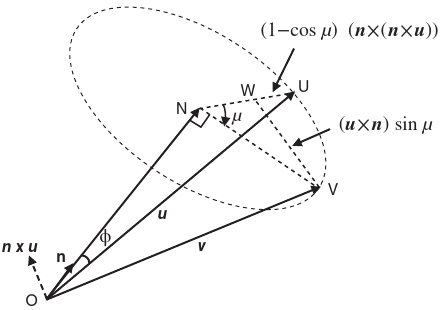
\includegraphics[width=0.5\textwidth, keepaspectratio]{figuras/figure1.2-1.png}\label{fig1.2-1}
    \caption{Rotação de um vetor}\label{fig:rotacao-de-um-vetor}
\end{figure}

Na figura acima, o vetor \(\mathbf{u}\) foi rotacionado para formar o vetor \(\mathbf{v}\) ao definirmos um eixo de rotação ao longo do vetor \(\mathbf{n}\) e realizarmos uma rotação pelo ângulo \(\mu\) ao redor de \(\mathbf{n}\). Estes dois vetores se somam a \(\mathbf{u}\) para obtermos \(\mathbf{v}\), e onde temos que:
    \begin{align*}
     \mathbf{v} &= \mathbf{u} + \left(1 - {\cos{\mu}}\right) \left(\mathbf{n}\!\times\!\left(\mathbf{n}\!\times\!\mathbf{u}\right)\right) - \left(\mathbf{n}\!\times\!\mathbf{u}\right){\sin{\mu}} \tag{1.2-5a}
    \end{align*}
    \begin{align*}
     \mathbf{v} = \left(1 - {\cos{\mu}}\right) \mathbf{n}\!\left(\mathbf{n}\cdot\mathbf{u}\right) + \mathbf{u}{\cos{\mu}} - \left(\mathbf{n}\!\times\!\mathbf{u}\right){\sin{\mu}} \tag{1.2-5b}
    \end{align*}

    As equações acima (1.2-5), às vezes chamadas de \textit{fórmula de rotação}, nos mostram que definindo \(\mathbf{n}\) e \(\mu\) podemos operar sobre \(\mathbf{u}\) com produtos escalares e vetoriais para obter a rotação desejada, independente de sistemas de coordenadas ou magnitude do ângulo.

    Partindo da figura acima, fazemos uma rotação muito pequena \(\delta\mu \ll 1 \text{rad}\), definindo \(\mathbf{v} = \mathbf{u} + \delta \mathbf{u}\), e, aplicando a equação (1.2-5\(a\)) obtemos:
\begin{equation*}
    \delta \mathbf{u} \approx -\!\sin(-\delta\mu)\mathbf{n}\!\times\!\mathbf{u} \approx (\mathbf{n}\!\times\!\mathbf{u})\delta\mu
\end{equation*}

Dividindo por \(\delta t\), no limite onde \(\delta t \rightarrow 0\), definindo \(\mathbf{\omega} \equiv \dot{\mu}\mathbf{n}\), obtemos:

\begin{equation*}
    \dot{\mathbf{u}} = \mathbf{\omega}\!\times\!\mathbf{u}\tag{1.4-1}
\end{equation*}

Esta equação relaciona a velocidade translacional da ponta do vetor \(\mathbf{u}\) ao vetor \(\mathbf{\omega}\). Este vetor \(\mathbf{\omega}\), que denominados \textit{vetor velocidade angular}, constitui-se de um vetor unitário  que define o eixo de rotação, multiplicado pela taxa de rotação. Este é um vetor livre, pode ser transladado paralelo a si mesmo, e axial, que mudaria de direção caso houvéssemos escolhido uma convenção de sentido horário para a rotação.

Dessa forma podemos associar \(\mathbf{\omega}\) ao sistema de coordenadas fixado no corpo, atribuindo índices que indicam que ele representa a velocidade angular do corpo em relação a outro determinado sistema.

Como vimos, a atitude de um corpo rígido pode ser descrita por uma matriz rotacional variante no tempo, e, pelo teorema de Euler\footnotemark{}, esse o corpo possui um único \emph{eixo instantâneo de rotação} ao qual o vetor velocidade angular é paralelo, e também único.

\footnotetext{\emph{``Euler's Theorem: The general displacement of a rigid body with one point fixed is a rotation about some axis.''} Para uma explicação a respeito, vide~\cite{Goldstein1980}, Capítulo 4.}

\section{Cinemática e Ângulos de Euler}

Um corpo em movimento pode mudar sua atitude, descrita em ângulos de Euler, ao longo do tempo, e neste sentido podemos falar de uma taxa de mudança de cada um desses ângulos de Euler ao longo do tempo. Essas taxas são coisa distintas, é preciso dizer, do vetor velocidade angular do corpo.

Para vincular as taxas de ângulos de Euler, que descrevem a mudança de atitude de um corpo, à sua velocidade angular, procedemos do seguinte modo. Definimos um quadro de referência \(F_{r}\) e um quadro do corpo \(F_{b}\) com vetor velocidade angular relativa \(\omega_{b/r}\) e uma sequencia de ângulos de Euler que define a atitude do corpo, ou seja, a orientação do sistema de coordenadas preso ao corpo em relação ao sistema de referência. Cada taxa de ângulos de Euler informa a direção e magnitude para um determinado vetor velocidade angular sobre um eixo de coordenadas em particular. Esses três vetores somados formam o vetor velocidade angular resultante do veículo cujas taxas de ângulos de Euler estamos tratando. Desse modo podemos encontrar os componentes do vetor velocidade angular resultante \cite{Stevens2016}.

Em outras palavras, movemos sobre a Terra um sistema de coordenada \(frd\) (\emph{``front'', ``right'', ``down''} - frente, direita, abaixo) preso no corpo, com o sistema \(ned\) (\emph{``north'', ``east'', ``down''} - norte, leste abaixo) fixo no quadro de referência, usando uma sequencia ``yaw-pitch-roll'' de ângulos de Euler do sistema \(ned\) para o sistema \(frd\). No caso das equações de Terra plana o sistema \(ned\) é fixado na Terra, e a velocidade angular relativa é aquela do corpo em relação à Terra. Não trataremos aqui do caso mais geral das equações com seis graus de liberdade onde sistema \(ned\) se move sobre a Terra.

As transformações de coordenadas são~\cite{Stevens2016}:

\begin{align*}
    \mathbf{\omega}^{frd}_{b/r} = \begin{bmatrix} \dot\phi \\ 0 \\0 \end{bmatrix}
    + C_{\phi} \begin{pmatrix}
        \begin{bmatrix} 0 \\ \dot\theta \\ 0 \end{bmatrix}
        + C_{\theta}\begin{bmatrix} 0 \\ 0 \\ \dot\psi \end{bmatrix}
    \end{pmatrix}
\end{align*}

\ldots sendo \(C_{\phi}\) e \(C_{\theta}\)  as rotações (anti-horárias) dos planos por cada ângulo de Euler em particular, conforme equação (1.3-10). Multiplicando as matrizes, teremos:

\begin{align} \tag{1.4-3}
    \mathbf{\omega}^{frd}_{b/r} \equiv \begin{bmatrix} P \\ Q \\ R \end{bmatrix}
    = \begin{bmatrix}
        1 & 0 & -\sin{\theta} \\
        0 & \cos{\phi} & \sin{\phi}\cos{\theta} \\
        0 & -\sin{\phi} & \cos{\phi}\cos{\theta}
    \end{bmatrix}
    \begin{bmatrix}
        \dot\phi \\
        \dot\theta \\
        \dot\psi
    \end{bmatrix}
\end{align}

\ldots sendo \(P\), \(Q\), \(R\), os componentes do vetor velocidade angular do corpo expressos no sistema \(frd\), respectivamente, rolagem (\emph{``roll''}), arfada (\emph{``pitch''}) e guinada (\emph{``yaw''}). A transformação inversa é dada por:

\begin{align} \tag{1.4-4}
    \begin{bmatrix}
        \dot\phi \\
        \dot\theta \\
        \dot\psi
    \end{bmatrix}
    =
    \begin{bmatrix}
        1 & \sin{\phi}\tan{\theta} & \cos{\phi}\tan{\theta} \\
        0 & \cos{\phi} & -\sin{\phi} \\
        0 & \frac{\sin{\phi}}{\cos{\theta}} & \frac{\cos{\phi}}{\cos{\theta}}
    \end{bmatrix}
    \begin{bmatrix}
        P \\ Q \\ R
    \end{bmatrix}
\end{align}

Para simplificar, definimos \(\mathbf{\Phi} \equiv \left[\phi \theta \psi \right]^T \) e reescrevemos  (1.4-4) assim:

\begin{equation} \tag{1.4-5}
    \dot{\mathbf{\Phi}} = H \left( \mathbf{\Phi} \right) \mathbf{\omega}^{frd}_{b/r}
\end{equation}

As equações (1.4-3) e (1.4-4) serão referidas como as equações cinemáticas de Euler, como faz~\cite{Stevens2016}. Note que as matrizes de coeficientes \emph{não são} matrizes ortogonais representando rotações ordinárias de coordenadas. Note ainda que as Equações (1.4-4) e (1.4-5) possuem uma singularidade quando  \(\theta = \pm \frac{\pi}{2}\). Ainda, se essas equações forem utilizadas em uma simulação, as taxas de ângulos de Euler podem integrar para ângulos fora do intervalos de ângulos de Euler, e portanto, seria necessário incluir uma lógica para lidar com essa situação no programa simulador. Não obstante, as equações cinemáticas de Euler são bastante empregadas em simulações.

\section{Derivada de um vetor em sistemas móveis}

Nesta seção deveremos obter as equações gerais para o movimento de um corpo no espaço tridimensional. Para generalizar a derivada de um vetor em relação em sistemas móveis obteremos \(^{a}\dot{\mathbf{p}}\) a partir da figura abaixo:
\begin{figure}[H]
    \centering
    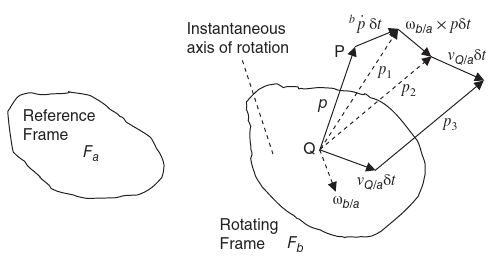
\includegraphics[width=0.5\textwidth, keepaspectratio]{figuras/figure1.4-1.png}\label{fig1.4-1}
    \caption{Derivada de um vetor em sistemas móveis.}
    \fonte{\cite{Stevens2016}}
\end{figure}

Os sistemas \(F_{b}\) e \(F_{a}\) têm velocidade angular relativa \(\mathbf{\omega}_{b/a}\). O ponto \(Q\), fixo em \(F_{b}\), traslada em relação a \(F_{a}\) a uma velocidade \(\mathbf{v}_{Q/a}\). Partindo de  \(Q\) nasce o vetor \(\mathbf{p}\). Observando a partir de \(F_{b}\) estabelecemos \(\mathbf{p}_{1}\) ao acrescentar o efeito \({^b\dot{\mathbf{p}}}\). Olhando a partir de \(F_{a}\) estabelecemos o vetor  \(\mathbf{p}_{2}\) ao somar, ainda, o efeito de \(\mathbf{\omega}_{b/a}\). A partir de \(F_{a}\), estabelecemos \(\mathbf{p}_{3}\) somando o efeito de \(\mathbf{v}_{Q/a}\), que, entretanto, não muda o comprimento ou direção de \(\mathbf{p}_{2}\). Portanto, para obtermos \(^{a}\dot{\mathbf{p}}\) devemos  comparar \(\mathbf{p}_{2}\) a \(\mathbf{p}\) quando \(\delta t \rightarrow 0\). Desse modo, no instante \(\delta t\), \(\mathbf{p}_{2} \!-\! \mathbf{p}\) temos:
\begin{equation*}
    \mathbf{p}_{2} - \mathbf{p} = {^{b}\dot{\mathbf{p}}} \delta t + \left( \mathbf{\omega}_{b/a} \! \times \!\mathbf{p} \right) \delta t
\end{equation*}

Dividindo por \(\delta t\) no limite em que \(\delta t \rightarrow 0\) resulta na equação\footnotemark{}:
\begin{equation*} \tag{1.4-2}
    {^{a}\dot{\mathbf{p}}} = {^{b}\dot{\mathbf{p}}} + {\mathbf{\omega}_{b/a} \! \times \!\mathbf{p}}
\end{equation*}

\footnotetext{``Equação de Coriolis''~\cite{Stevens2016},~\cite{Blakelock1991}.}

Dentre as propriedades do vetor velocidade angular destacamos\footnotemark{}:
\begin{enumerate}[label=\alph*)]
\item É único e relaciona as derivadas de um vetor tomadas em dois sistemas.
\item Satisfaz a condição de movimento relativo \(\mathbf{\omega}_{b/a} = - \mathbf{\omega}_{a/b}\).
\item É aditivo entre sistemas, ou seja, \(\mathbf{\omega}_{c/a} = \!\mathbf{\omega}_{c/b} + \mathbf{\omega}_{b/a}\) (não vale para aceleração angular).
\item Sua derivada é ambos os sistemas , \({^{a}\dot{\mathbf{\omega}}_{b/a}} = {^{b}\dot{\mathbf{\omega}}_{a/b}} \) .
\end{enumerate}
\footnotetext{Seguindo \cite{Stevens2016}}.

Ainda, derivada de um vetor em um quadro pode ser encontrada a partir das derivadas dos seus componentes expressas em um sistema fixo no mesmo quadro, por exemplo:
\begin{equation*}
    \mathbf{v}^{a\!f} = \begin{bmatrix} v_{x} & v_{y} & v_{z} \end{bmatrix}^{T}
\end{equation*}

\section{Velocidade e Aceleração em quadros móveis}

Encontraremos velocidade e aceleração do ponto \(P\), situado em \(\mathbf{p}\), que se move em relação a \(F_{a}\) e \(F_{b}\), onde fixamos \(O\) and \(Q\), respectivamente, os quais também se movem em relação um ao outro. Na figura abaixo, relacionamos os vetores posição, tomamos suas derivadas no quadro de referência\footnotemark{} \(F_{a}\),  determinando a velocidade. Usando \(\mathbf{v}\) para um vetor velocidade, aplicamos a equação de Coriolis obtendo~\cite{Stevens2016}:
\footnotetext{A escolha do quadro \(F_{a}\) como referência é arbitrária.}
\begin{figure}[H]
    \centering
    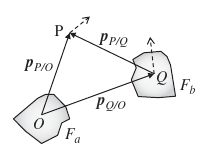
\includegraphics[width=0.25\textwidth, keepaspectratio]{figuras/figure1.5-1.png}
    \label{fig1.5-1}
    \caption{Velocidade e aceleração em quadros móveis}
    \fonte{\cite{Stevens2016}}
\end{figure}
\begin{align}
    \mathbf{p}_{P/O}             &= \mathbf{p}_{Q/O} + \mathbf{p}_{P/Q} \tag{1.5-1} \\
    {^{a}\dot{\mathbf{p}}_{P/O}} &= {^{a}\dot{\mathbf{p}}_{Q/O}} + {^{a}\dot{\mathbf{p}}_{P/Q}} \tag{1.5-2} \\
    \mathbf{v}_{P/a}             &= \mathbf{v}_{Q/a} + \left( \mathbf{v}_{P/b} + \mathbf{\omega}_{b/a}\!\times\!\mathbf{p}_{P/Q} \right) \tag{1.5-3}
\end{align}

Rearranjando para destacar os temos em parênteses\footnotemark{}:
\begin{equation*}
    \mathbf{v}_{P/a} = \mathbf{v}_{P/b} + \left( \mathbf{v}_{Q/a} + \mathbf{\omega}_{b/a}\!\times\!\mathbf{p}_{P/Q} \right),
\end{equation*}
\footnotetext{O termo em parênteses corresponde à chamada \textit{velocidade de transporte de \(P\) no quadro \(F_{a}\)} (a velocidade em \(F_{a}\) de um ponto fixo em \(F_{b}\) coincidente com \(P\)).}

Para a aceleração derivamos (1.5-3) em \(F_{a}\). Velocidades em \(F_{a}\) se tornam acelerações em \(F_{a}\); A velocidade em \(F_{b}\) é derivada pela Equação de Coriolis; A produto vetorial é derivado pela ``regra do produto vetorial''\footnotemark{}; A derivada da velocidade angular é um vetor aceleração angular designado \(\mathbf{\alpha}\). Seja \(\mathbf{a}\) a aceleração translacional em (1.5-3), obtemos:
\begin{equation*}
    \mathbf{a}_{P/a} = \mathbf{a}_{Q/a} + \left(\mathbf{a}_{P/b} + \mathbf{\omega}_{b/a}\!\times\!\mathbf{v}_{P/b}\right) + {{\mathbf{\alpha}_{b/a}}\!\times\!{\mathbf{p}_{P/Q}}} + {\mathbf{\omega}_{b/a}}\!\times\!{\left({\mathbf{v}_{P/b}} + {{\mathbf{\omega}_{b/a}}\!\times\!{\mathbf{p}_{P/Q}}}\right)}
\end{equation*}
\footnotetext{??? TODO incluir nos anexos a Regra do Produto Vetorial.}

Reorganizando, destacamos aceleração ``\emph{de transporte}'', ``\emph{centrípeta}'' e ``\emph{de Coriolis}'':
\begin{equation*}
    \mathbf{a}_{P/a} = \mathbf{a}_{P/b} + \overbrace{\mathbf{a}_{Q/a} + {{\mathbf{\alpha}_{b/a}}\!\times\!{\mathbf{p}_{P/Q}}} + \underbrace{{{\mathbf{\omega}_{b/a}}\!\times\!{\left({\mathbf{\omega}_{b/a}}\!\times\!{\mathbf{p}_{P/Q}}\right)}}}_{\text{aceleração centrípeta}}}^{\text{aceleração de transporte}} + \underbrace{{2\mathbf{\omega}_{b/a}\!\times\!\mathbf{v}_{P/b}}}_{\text{aceleração de Coriolis}} \tag{1.5-4}
\end{equation*}


Os termos \(\mathbf{a}_{P/a}\) e \(\mathbf{a}_{P/b}\), denominados \emph{aceleração total} e \emph{aceleração relativa}, são expressos nos quadros de referência e secundário, respectivamente. Notamos o surgimento do termo \textit{aceleração de Coriolis}, a ser examinado mais adiante. Se fixamos \(P\) no quadro \(F_{b}\), nos resta apenas \textit{aceleração de  transporte}, definida como a aceleração expressa em \(F_{a}\) de um ponto fixo em \(F_{b}\) instantaneamente coincidente com \(P\). A aceleração de transporte expressa os efeitos do movimento de \(F_{b}\), em termos de aceleração do ponto \(Q\), da velocidade angular e da aceleração angular do quadro~\cite{Stevens2016}.


Por exemplo, um acelerômetro fixo num robô móvel, de corpo rígido, não se move em relação ao quadro do corpo do robô, restando apenas os termos relativos à velocidade e aceleração de transporte nas equações 1.5-3 e 1.5-4, respectivamente. A aceleração para o sensor no ponto \(P\), de posição \(\mathbf{p}_{P/Q}\) em relação a ponto \(Q\) fixo no quadro do robô, denotando \(a\) and \(b\) os quadros de referência e do robô, respectivamente, é dada por \cite{Stevens2016}:
\begin{equation*}
    {\mathbf{a}_{P/a}} = {\mathbf{a}_{Q/a}} + {\mathbf{\alpha}_{b/a}}\!\times\!{\mathbf{p}_{P/Q}} + {\mathbf{\omega}_{b/a}}\!\times\!\left({\mathbf{\omega}_{b/a}}\!\times\!{\mathbf{p}_{P/Q}}\right)
\end{equation*}

Aplicando para um corpo sobre a Terra, sejam \(F_{i}\)  e  \(F_{e}\) quadros de referencia inercial e fixo na Terra, respectivamente, e pontos \(Q\) e \(O\) coincidentes no centro de massa da Terra (sem aceleração translacional), o \(\mathbf{p}_{P/Q}\) é um vetor posição geocêntrico, e \(\mathbf{a}_{Q/a}=0\). Considerando que a Terra gira a uma velocidade angular constante, a derivada de \(\mathbf{\omega}_{b/a}\) também desaparece. Restam a aceleração relativa, a centrípeta e a de Coriolis na equação que relaciona a aceleração verdadeira (inercial) à aceleração relativa, para aplicar as leis de Newton no movimento de um ponto \(P\) sobre a Terra~\cite{Stevens2016}:
\begin{equation*} \tag{1.5-5}
    {\mathbf{a}_{P/i}} = {\mathbf{a}_{P/e}} + {\mathbf{\omega}_{e/i}}\!\times\!\left({\mathbf{\omega}_{e/i}}\!\times\!{\mathbf{p}_{P/O}}\right) + 2\mathbf{\omega}_{e/i}\!\times\!\mathbf{v}_{P/e}
\end{equation*}

Neste sentido, para uma partícula de massa \(m\) situada em \(P\), a aceleração relativa \(\mathbf{a}_{P/e}\) corresponde uma ``força aparente'' sobre a partícula que produz a trajetória vista por um observador estacionário na Terra. A aceleração verdadeira \(\mathbf{a}_{P/i}\) correspondem às `` forças verdadeiras'' (como gravitação e arraste).  Escrevendo (1.5-5) em termos de forças, onde destacamos a \textit{força centrífuga} normal ao vetor velocidade angular, e a \textit{força de Coriolis}\footnotemark{} que fará uma trajetória balística sobre a Terra curvar-se à esquerda ou à direita~\cite{Stevens2016}:
\begin{equation*}
    \text{Força aparente} = \text{força verdadeira} - \underbrace{m \left[{\mathbf{\omega}_{e/i}}\!\times\!\left({\mathbf{\omega}_{e/i}}\!\times\!{\mathbf{p}_{P/O}}\right)\right]}_{\text{força centrífuga}} - \underbrace{m \left( 2{\mathbf{\omega}_{e/i}}\!\times\!{\mathbf{v}_{P/e}}\right)}_{\text{força de Coriolis}}
\end{equation*}

Força verdadeira (\(F\)) é a soma das \textit{forças de contato}. A força do  \textit{campo gravitacional da Terra} corresponde a \(m\mathbf{G}\). O vetor gravidade da Terra (\(g\)) é dado por {\(\mathbf{g}~=~\mathbf{G}~-~\text{aceleração centrípeta}\)}. Desse modo, reescrevendo a equação (1.5-5) para um corpo rígido de massa \(m\), obtemos~\cite{Stevens2016}:
\begin{equation*} \tag{1.5-6}
    \mathbf{a}_{P/e} = \frac{F}{m} + g - {2 \mathbf{\omega}_{e/i}}\!\times\!{\mathbf{v}_{P/e}}
\end{equation*}

\footnotetext{A aceleração de Coriolis será significativa para deslocamento em altas velocidades. Para ilustrar, para que a aceleração de Coriolis tenha a mesma magnitude da aceleração centrípeta, a \(45^{\circ}\) de latitude, um veículo deve deve mover-se a 2365.2 km/h. Nessa velocidade, embora a aceleração de Coriolis ainda seja pequena comparada a \(\mathbf{g}\), causa uma diferença de posição que cresce com o tempo~\cite{Stevens2016}.
\begin{align*}
    &2 \! \begin{vmatrix}{\mathbf{\omega}_{e/i}}\end{vmatrix} \begin{vmatrix}{\mathbf{v}_{cm/e}}\end{vmatrix}\sin\!{\left({45^{\circ}}\right)} = {\begin{vmatrix}{\mathbf{v}_{cm/e}}\end{vmatrix}^{2}} / {r_{E}} \\
    &\begin{vmatrix}{\mathbf{v}_{cm/e}}\end{vmatrix} = {\sqrt{2}}{r_{E}} \begin{vmatrix} {\mathbf{\omega}_{e/i}}\end{vmatrix} \approx 657\text{m/s} \left(2365.2\text{km/h}\right)
\end{align*}
}


\section{Gravitação e acelerômetros}

Um acelerômetro mede, indiretamente\footnotemark{}, a força \(\mathbf{F}\) que equilibra uma \emph{massa de prova} com o encapsulamento. Com o campo gravitacional atuando na massa de prova \(m\), seja \(\mathbf{F}/m\) a força por unidade de massa aplicada à massa de prova, chamada de força específica, \(\mathbf{f}\) determinamos a aceleração \(\mathbf{a}\) da massa de prova~\cite{Stevens2016}:
\begin{equation*}
    \mathbf{a} = \dfrac{\mathbf{F}}{m} + \mathbf{G} \equiv \mathbf{f} + \mathbf{G}.
\end{equation*}
\footnotetext{Para detalhes sobre acelerômetros,~\cite{Weston2004},~\cite{Wang2021} e~\cite{Haoran2019}.}

Com a calibração determinamos o \textit{fator de escala}, entre a quantidade de saída do sinal à força específica\cite{Stevens2016}:
\begin{equation*} \tag{1.6-28}
    \text{Sinal de saída do acelerômetro} = s \mathbf{f} = s \left(\mathbf{a} - \mathbf{G} \right)
\end{equation*}

Quando um acelerômetro, com vetor de posição geocêntrico\footnotemark{} \(\mathbf{p}\), está estacionário em relação à Terra, a leitura de aceleração corresponde a~\cite{Stevens2016}:
\begin{align*}
    \mathbf{a} &= {\mathbf{\omega}_{e/i}}\!\times\!\left({\mathbf{\omega}_{e/i}}\!\times\!{\mathbf{p}}\right) \\
    \mathbf{f} &= \mathbf{a} - \mathbf{G} = -\!{\mathbf{g}} \tag{1.6-29}
\end{align*}
\footnotetext{A navegação inercial exige um modelo para \(\mathbf{G}\) em função da posição. Numa posição diferente, o acelerômetro deve ser corrigido para a gravidade local e pela aceleração centrípeta. Para um acelerômetro fixado em um veículo que se move em relação à Terra, devemos ainda calcular a aceleração de transporte para relacionar a leitura do acelerômetro com a aceleração do veículo~\cite{Stevens2016}.}

Para um acelerômetro com três eixos ortogonais \(x\), \(y\) e \(z\), situado num ponto \({P}\) fixado no quadro \({F}_{frd}\) do corpo de um robô, com vetor de posição geocêntrico \(\mathbf{p}\), designamos \(\mathbf{G}_{p}\) o vetor projeção da força nos elementos sensores, \(\mathbf{g}\) o vetor aceleração da gravidade expresso em múltiplos da \emph{gravidade padrão}, \(\mathbf{a}\) a aceleração do corpo tomada no quadro de referência da Terra, e \({C}_{frd/ned}\) a matriz de rotação do quado \(frd\) em relação ao \(ned\), obtendo a equação:
\begin{equation*}
    {\mathbf{G}}_p = \begin{bmatrix} {G}_{px} \\ {G}_{py} \\ {G}_{pz} \end{bmatrix} = {C}_{frd/ned}\left(\mathbf{g} - {\mathbf{a}}\right)
\end{equation*}

Assumindo que o robô não acelera (\(\mathbf{a}\approxeq0\)) e que na orientação inicial os eixos ``abaixo'' no sistemas \(frd\) e \(ned\) estão alinhados, com o vetor \(\mathbf{g}\) projetando apenas no eixo \(z\) do acelerômetro, então a equação acima se transforma em:
\begin{align*}
    {\mathbf{G}}_p &= \begin{bmatrix}
        c\theta c\psi   & c\theta s\psi & -s\theta    \\
        \left(-c\phi s\psi + s\phi s\theta c\psi \right)
        &  \left( c\phi c\psi + s\phi s\theta s\psi \right)
        &  s\phi c\theta                                 \\
        \left( s\phi s\psi + c\phi s\theta c\psi \right)
        &  \left( -s\phi c\psi + c\phi s\theta s\psi \right)
        & c\phi c\theta
    \end{bmatrix} \begin{bmatrix} 0 \\ 0 \\ 1 \end{bmatrix} = \begin{bmatrix} -\sin{\theta} \\ \cos{\theta}\sin{\phi} \\ \cos{\theta}\cos{\phi} \end{bmatrix}
\end{align*}

A equação acima depende apenas de \(\theta\) e \(\phi\), pois na primeira rotação por \(\psi\) sobre o eixo \emph{abaixo} o vetor \(\mathbf{g}\) permanece alinhado ao eixo \(z\) do sensor. Um acelerômetro, portanto, é insensível a essa rotação por \(\psi\), e não serve para determinar o ângulo de guinada\footnotemark{}. Normalizando as leituras, isolamos \(\theta\) e \(\phi\) por identidades trigonométricas sobre a projeção da gravidade (\(\mathbf{g}\)) nos eixos do sensor~\cite{freescaleAN3461}:
\begin{equation*}
    \frac{{\mathbf{G}}_{p}}{\lVert{{\mathbf{G}}_{p}}\rVert} =
    \frac{1}{\sqrt{{{{G}_{px}}^{2}} + {{{G}_{py}}^{2}} + {{G}_{pz}}^{2}}} \begin{bmatrix} {G}_{px} \\ {G}_{py} \\ {G}_{pz} \end{bmatrix}
    = \begin{bmatrix} -\sin{\theta} \\ \cos{\theta}\sin{\phi} \\ \cos{\theta}\cos{\phi} \end{bmatrix} \\
\end{equation*}
\begin{align*}
    \tan{\phi}_{xyz} &= \frac{G_{py}}{G_{pz}} \\
    \tan{\theta}_{xyz} &= \frac{-G_{px}}{{G_{py}\sin{\phi}}+{{{G}_{pz}}\cos{\phi}}} = \frac{-G_{px}}{\sqrt{{{G_{py}}^{2}}+{{{G}_{pz}}^2}}}
\end{align*}

Empregando funções trigonométricas inversas, obtemos \(\theta\) e \(\phi\):
\begin{align*}
{\phi}_{xyz} &= \tan^{-1}\left(\frac{G_{py}}{G_{pz}}\right) \\
{\theta}_{xyz} &= \tan^{-1}\left(\frac{-G_{px}}{\sqrt{{{G_{py}}^{2}}+{{{G}_{pz}}^2}}}\right) \\
\end{align*}
\footnotetext{Para \(\psi\) poderíamos empregar um magnetômetro~\cite{freescaleAN4248}.}

\ldots e definimos o intervalo de validade\footnotemark{} como fizemos para a matriz rotacional:
\begin{align*}
    -\pi  < \phi \leq \pi \\
    -\frac{\pi}{2} \leq \theta \leq \frac{\pi}{2} \\
\end{align*}
\footnotetext{Nas equações há uma região de instabilidade onde \(\mathbf{G}_{py}\) e \(\mathbf{G}_{pz}\) tendem a zero, quando o eixo \(x\) do acelerômetro encontra-se alinhado verticalmente para cima ou para baixo. Nas proximidades dessa região o cálculo da tangente inversa é dominado pelo ruído do sensor, produzindo uma estimativa de ângulo praticamente aleatória. Fisicamente, quando o eixo \(x\) do acelerômetro está na vertical, o ângulo de rolagem \(\phi\) corresponde a uma rotação sobre o vetor do campo gravitacional, para a qual o acelerômetro é insensível. Algun artifícios podem minimizar a instabilidade~\cite{freescaleAN3461}}.

%Ainda sobre o mesmo robô, que não acelera (\(\mathbf{a}\approxeq0\)), mas muda a sua atitude do instante \({t}_{a}\) para \({t}_{b}\), com projeções \(\mathbf{G}_{{p}_{\left[{t}_{a}\right]}\) e \(\mathbf{G}_{{p}_{\left[{t}_{b}\right]}}\), respectivamente, do vetor contante \(\mathbf{g}\) sobre os eixos \(x\), \(y\) e \(z\) do mesmo acelerômetro, estimamos as atitudes \({\Phi}_{\left[{t}_{a}\right]}\) e \({\Phi}_{\left[{t}_{b}\right]}\). Pelo teorema de Euler, aplicamos os produtos escalar e vetorial para estimar o ângulo e o eixo da rotação que leva o vetor \(g\) da projeção \(\mathbf{G}_{{p}_{\left[{t}_{a}\right]}\) à \(\mathbf{G}_{{p}_{\left[{t}_{b}\right]}}\):
%
%\begin{equation*}
%    \mathbf{a} . \mathbf{b} &= \|\mathbf{a}\|\|\mathbf{b}\|\cos{\alpha}\\
%\end{equation*}
%\begin{equation*}
%    \mathbf{a}\times\mathbf{b} &= \|\mathbf{a}\|\|\mathbf{b}\|{\hat{\mathbf{n}}}\sin{\alpha}\\
%\end{equation*}
%
\section{Dinâmica de corpo rígido}

??? em fase de adaptação usando \cite{Stevens2016}

Nesta seção finalmente juntamos as idéias e equações das seções anteriores para obter um conjunto de equações de estado que descreve o o movimento com seis graus de liberdade de um verículo aeroespacial rígido (definido sistema \(F_{b}\)). Lidamos primeiro com o movimento angular do veículo em relação a torques oriundos de forças aerodinâmicas, empuxo, ou quaisquer outras, cujas linhas de ação não passam pelo centro de massa do veículo. Empregando o centro de masssa como ponto de referência a dinâmica rotacional da aeronave pode ser separada da dinâmica translacional (Wells, 1967): portanto utilizamos um sistema de coordenadas fixo no corpo \(bf\) com origem no centro de massa para calcular os momentos sobre a origem. Um vetor torque não nulo produz uma taxa de mudança do vetor momento angular, mas então, para relacionar o momento angular à distribuição de massa de um corpo em específico, devemos utilizar o sistema de coordenada \(bf\) e alternar para equações matriciais para obter os componentes do vetor aceleração angular. Componentes de aceleração angular integram para componentes velocidade angular, mas então os três graus de liberdade no deslocamento angular são obtidos a partir de equações não lineares como as equações de Euler (1.4-4). Para uma aeronave, o sistem \(bf\) normalmente é o sistema \(frd\) descrito na Seção 1.3. 

As equações de movimento translacional são mais diretas, a aceleração do centro de massa do veículo é obtida da soma vetorial das várias forças, cujas linhas de ação não precisam passar pelo centro de massa porque o efeito de qualquer torsão foi incorporada nas equações do momento. As equações são expressas em termos de movimento relativo à Terra e introduzem os termos de Coriolis e centrípeta como de costume. Efeitos aerodinâmicos e de empuxo dependem dependem do movimento relativo à atmosfera envolvente, então quando a atmosfera se move em relação à Terra, introduzimos equações auxiliares para calcular os \emph{ventos relativos}.

\subsection{Equações do movimento para Terra plana}

??? em fase de adaptação usando \cite{Stevens2016}

Como explicado acima, as equações de Terra plana não são servem para determinar com precisão a posição sobre a Terra, mas são amplamente utilizadas em simulações para estudar o desempenho e o comportamento dinâmico de aeronaves e são empregadas para derivar modelos lineares de espaço de estados para estudos analíticos e projeto de sistemas de controle. Os pressupostos para a as equações de terra plana serão agora formalmente listados:

\begin{enumerate}
    \item A Terra é um referencial inercial
    \item Posição é medida no sistema de coordenadas do plano tangente \(tp\).
    \item O vetor gravidade é normal ao plano tangente e constante em magnitude.
\end{enumerate}

Por consequência, também presumimos:

\begin{enumerate}
    \item Altura acima do plano tangente é uma boa aproximação para a altura verdadeira acima da superfície da Terra, e a projeção horizontal do vetor posição oferece uma boa aproximação à distância percorrida sobre a superfície da Terra (o que é razoável até algumas centenas de milhas a partir da origem do plano tangente).
    \item A atitude do veículo no sistema do plano tangente é uma boa aproximação à verdadeira atitude geográfica na posição do veículo.
\end{enumerate}

A equação (1.7-16) já impõe a primeira assunção, e a variável de estado posição já refere-se à origem do plano tangente. Agora devemos escolher sistemas de coordenadas para as variáveis nas equações de estado e nos preparar para calcular a matriz de rotação para converter de um sistema para outro quando necessário.

Um sistema \(frd\) fixo em \(F_{b}\) é muito conveniente para derivar o vetor velocidade em \(F_{b}\), para forças aerodinâmicas e propulsoras, e para o vetor velocidade angular do veículo (que utiliza os eixos do componentes em eixos do corpo nas equações de movimento angular). Esta escolha é menos oportuna para o vetor \(\mathbf{g}\) e para o vetor velocidade angular da Terra, que são conhecidos em sistemas de coordenadas fixos à Terra e devem ser rotacionados para o sistema do corpo usando uma matriz rotacional obtida a partir das equações de estado. Nas equações de Terra plana, a mudança de atitude do veículo é quase sempre adequadamente modelada com as simples equações cinemáticas de Euler (1.4-4). Estas relacionam o sistema \(frd\) fixo no corpo ao sistema \(ned\), sendo que o sistema \(ned\) corresponde ao plano tangente \(tp\) fixo na Terra. Os ângulos de Euler podem então serem usados para obter a matriz de rotação \(C_{frd/ned}\), que deve ser empregada antes para que possamos calcular as equações de posição e velocidade.

O conjunto das equações para seis graus de liberdade será completado adicionando a equação de estado da velocidade angular (1.7-5), com \(\mathbf{\omega}_{b/i} \equiv \mathbf{\omega}_{b/e}\) como variável de estado. Então o vetor de estado se torna

\begin{align*}\tag{1.7-17}
    X^{T} =
    \begin{bmatrix}
    \left( \mathbf{p}^{tp}_{cm/O} \right) &
    \mathbf{\Phi}^{T} {\left(\mathbf{v}^{frd}_{cm/e}\right)}^{T} &
    {\left(\mathbf{\omega}^{frd}_{b/e} \right)}^{T}
    \end{bmatrix}
\end{align*}

Usando o valor das variáveis de estado, calculamos o valor das derivadas do estado a seguir. A matriz de rotação é calculada antes da equações de estado da posição e velocidade como referido acima. Derivadas de ângulos aerodinâmicos podem ser calculadas a partir das derivadas de velocidade translacional, portanto a equação de velocidade translacional é situada antes da equação de velocidade angular, onde aquelas derivadas são mais significativas (detalhamos no Capítulo 3) então temos o seguinte conjunto de equações:

\begin{align*}\tag{1.7-18}
    C_{frd/tp} &= fn \left( \Phi \right) \\
    \dot{\Phi} &=  H \left( \Phi \right) {\mathbf{\omega}^{frd}_{b/e}} \\
    {^{e}{\dot{\mathbf{p}}^{tp}_{cm/Q}}} &= {C_{tp/frd}}{\mathbf{v}^{frd}_{cm/e}} \\
    {^{b}{\dot{\mathbf{v}}^{frd}_{cm/e}}} &= \textstyle{\frac{1}{m}} {\mathbf{F}^{frd}} + {C_{frd/tp}}{\mathbf{g}^{tp}} - {\tilde{\mathbf{\omega}}^{frd}_{b/e}} {\mathbf{v}^{frd}_{cm/e}} \\
    { ^{b}{\dot{\mathbf{\omega}}^{frd}_{b/e}}} &= {\left( J^{frd} \right)}^{-1}
    \begin{bmatrix}
        \mathbf{M}^{frd} & -{\tilde{\mathbf{\omega}}^{frd}_{b/e}} {J^{frd}} & {\mathbf{\omega}^{frd}_{b/e}}
    \end{bmatrix}
\end{align*}

A equações de Terra plana com seis graus de liberdade contidas em (1.7-18) são doze equações diferenciais escalares, acopladas, não lineares, e uma equação auxiliar. O acoplamento ocorre porque a aceleração angular integra para velocidade angular, que determina as taxas de ângulos de Euler, que por sua vez determinam a matriz de rotação. A matriz de rotação está envolvida nas equações de posição e velocidade, posição (o componente altitude) e velocidade determinam os efeitos aerodinâmicos que determinam a aceleração angular. O acoplamento também está presente através da velocidade translacional. Estas inter-relações ficarão mais aparentes no Capítulo 2.

Para completar as assunções de terra Plana, \(\mathbf{g}\) em coordenadas do plano tangente será

\begin{equation*}
\mathbf{g}^{tp} = {\begin{bmatrix} 0 & 0& g_{D} \end{bmatrix}}^{T}
\end{equation*}

com o componente abaixo, \(\mathbf{g}_{D}\) igual à gravidade padrão (\(9.80665 \textrm{m/s}^{2}\)) ou seu valor local. 

%Cálculos aerodinâmicos requerem a equação para o vetor velocidade relativo à atmosfera envolvente [da equação (1.7-14)]:
%
%\begin{equation*}\tag{1.7-19}
%    \mathbf{v}^{frd}_{rel} =  \mathbf{v}^{frd}_{cm/e} - \mathbf{C}_{frd/tp} \mathbf{v}^{tp}_{W/e}
%\end{equation*}
%
%Para calcular os efeitos aerodinâmicos necessitamos de algumas outras equações adicionais que serão introduzidas no Capítulo 2.
%
